% ============================================================
%  OPC UA — INDUSTRIAL COMMUNICATION PROTOCOL STUDY GUIDE
%  For SCADA Automation Engineers
%  Covers all 10 chapters: Intro through Lab & Tools
% ============================================================
\documentclass[12pt,twoside,openright]{memoir}

% ── Encoding & fonts ─────────────────────────────────────────
\usepackage[T1]{fontenc}
\usepackage[utf8]{inputenc}
\usepackage{lmodern}
\usepackage{microtype}
\usepackage{palatino}
\usepackage[scaled=0.85]{beramono}

% ── Page geometry ────────────────────────────────────────────
\usepackage[
  top=1.25in, bottom=1.25in,
  inner=1.5in, outer=1.0in,
  marginparwidth=0.8in, marginparsep=0.1in
]{geometry}

% ── Colors ───────────────────────────────────────────────────
\usepackage[dvipsnames,svgnames,x11names]{xcolor}
\definecolor{opcuanavy}{HTML}{0D2137}
\definecolor{opcuablue}{HTML}{1565C0}
\definecolor{opcuacyan}{HTML}{0097A7}
\definecolor{opcuaorange}{HTML}{E65100}
\definecolor{opcuagreen}{HTML}{2E7D32}
\definecolor{opcuared}{HTML}{C62828}
\definecolor{opcuayellow}{HTML}{F9A825}
\definecolor{rowlight}{HTML}{EFF6FF}
\definecolor{rowdark}{HTML}{DBEAFE}
\definecolor{codebg}{HTML}{F8F9FA}
\definecolor{frameborder}{HTML}{455A64}
\definecolor{covergray}{HTML}{ECEFF1}
\definecolor{warnbg}{HTML}{FFF3E0}
\definecolor{fieldbg}{HTML}{E8F5E9}
\definecolor{securityred}{HTML}{FFEBEE}
\definecolor{securitygreen}{HTML}{E8F5E9}
\definecolor{securityamber}{HTML}{FFF8E1}

% ── Graphics & TikZ ──────────────────────────────────────────
\usepackage{graphicx}
\usepackage{tikz}
\usetikzlibrary{positioning,shapes.geometric,arrows.meta,decorations.pathreplacing,
                matrix,fit,backgrounds,calc,patterns,shadows.blur}
\usepackage{pgfplots}
\pgfplotsset{compat=1.18}

% ── Tables ───────────────────────────────────────────────────
\usepackage{booktabs}
\usepackage{tabularx}
\usepackage{array}
\usepackage{multirow}
\usepackage{colortbl}
\newcolumntype{L}[1]{>{\raggedright\arraybackslash}p{#1}}
\newcolumntype{C}[1]{>{\centering\arraybackslash}p{#1}}
\newcolumntype{R}[1]{>{\raggedleft\arraybackslash}p{#1}}

% ── Callout boxes (tcolorbox) ─────────────────────────────────
\usepackage[most,listings]{tcolorbox}

\newtcolorbox{keyconcept}[1][]{
  enhanced, breakable,
  colback=opcuablue!8, colframe=opcuablue, arc=4pt,
  fonttitle=\bfseries\sffamily\color{white}, title={Key Concept},
  attach boxed title to top left={yshift=-2mm, xshift=6mm},
  boxed title style={colback=opcuablue, arc=3pt},
  #1
}

\newtcolorbox{warningbox}[1][]{
  enhanced, breakable,
  colback=warnbg, colframe=opcuaorange, arc=4pt,
  fonttitle=\bfseries\sffamily\color{white}, title={WARNING},
  attach boxed title to top left={yshift=-2mm, xshift=6mm},
  boxed title style={colback=opcuaorange, arc=3pt},
  #1
}

\newtcolorbox{example}[2][]{
  enhanced, breakable,
  colback=fieldbg, colframe=opcuagreen, arc=4pt,
  fonttitle=\bfseries\sffamily\color{white}, title={Example: #2},
  attach boxed title to top left={yshift=-2mm, xshift=6mm},
  boxed title style={colback=opcuagreen, arc=3pt},
  #1
}

\newtcolorbox{fieldgotcha}[1][]{
  enhanced, breakable,
  colback=opcuared!6, colframe=opcuared, arc=4pt,
  fonttitle=\bfseries\sffamily\color{white}, title={Field Gotcha},
  attach boxed title to top left={yshift=-2mm, xshift=6mm},
  boxed title style={colback=opcuared, arc=3pt},
  #1
}

\newtcolorbox{protip}[1][]{
  enhanced, breakable,
  colback=opcuayellow!15, colframe=opcuayellow!70!black, arc=4pt,
  fonttitle=\bfseries\sffamily, title={Pro Tip},
  attach boxed title to top left={yshift=-2mm, xshift=6mm},
  boxed title style={colback=opcuayellow!70!black, arc=3pt},
  #1
}

% ── Code listings ─────────────────────────────────────────────
\lstset{
  basicstyle=\ttfamily\small,
  backgroundcolor=\color{codebg},
  frame=single, framerule=0.4pt, frameround=tttt,
  rulecolor=\color{frameborder},
  breaklines=true, breakatwhitespace=true,
  tabsize=2, showstringspaces=false,
  keywordstyle=\color{opcuablue}\bfseries,
  commentstyle=\color{opcuagreen}\itshape,
  stringstyle=\color{opcuaorange},
}

% ── Fonts & headings ──────────────────────────────────────────
\usepackage{fontawesome5}
\usepackage{titlesec}
\titleformat{\chapter}[display]
  {\normalfont\huge\bfseries\color{opcuanavy}}
  {\chaptertitlename\ \thechapter}{20pt}{\Huge}
\titleformat{\section}
  {\normalfont\Large\bfseries\color{opcuablue}}
  {\thesection}{1em}{}
\titleformat{\subsection}
  {\normalfont\large\bfseries\color{opcuacyan}}
  {\thesubsection}{1em}{}

% ── Hyperlinks ────────────────────────────────────────────────
\usepackage[
  colorlinks=true,
  linkcolor=opcuablue,
  urlcolor=opcuacyan,
  citecolor=opcuagreen,
  bookmarks=true,
  pdfauthor={Ricardo Barbosa},
  pdftitle={OPC UA Industrial Communication Protocol Study Guide},
]{hyperref}

% ── Header/footer ────────────────────────────────────────────
\pagestyle{headings}
\makeoddhead{headings}{}{}{\small\textit{OPC UA Study Guide}}
\makeevenhead{headings}{\small\textit{Ricardo Barbosa}}{}{}

% ─────────────────────────────────────────────────────────────
\begin{document}

% ── Cover ─────────────────────────────────────────────────────
\begin{titlingpage}
  \pagecolor{opcuanavy}
  \color{white}
  \vspace*{2cm}
  \begin{center}
    {\fontsize{48}{56}\selectfont\bfseries OPC UA}\\[0.5em]
    {\Large Industrial Communication Protocol}\\[0.3em]
    {\large Study Guide}\\[3cm]
    \textcolor{opcuacyan}{\rule{0.6\textwidth}{2pt}}\\[1.5cm]
    {\large For SCADA Automation Engineers}\\[0.5em]
    {\normalsize Secure Channel $\cdot$ Address Space $\cdot$ Subscriptions $\cdot$ Certificates}\\[2cm]
    {\large\bfseries Ricardo Barbosa}\\[0.3em]
    {\small NERC-Certified EDF Operator}\\[0.3em]
    {\small MS Artificial Intelligence, Johns Hopkins University}\\[2cm]
    {\small\textcolor{opcuacyan}{May 2026}}
  \end{center}
\end{titlingpage}
\nopagecolor

\clearpage

% ── Table of Contents ─────────────────────────────────────────
\tableofcontents
\clearpage

% =============================================================
\chapter{What Is OPC UA?}
% =============================================================

OPC UA --- Unified Architecture --- is an industrial communication standard published by the OPC Foundation in 2008.
It defines how machines, sensors, PLCs, SCADA systems, and enterprise software exchange data in a platform-independent,
secure, and structured way.

\begin{keyconcept}
OPC UA is a platform-independent, secure, structured data exchange protocol for industrial automation. It replaced
OPC Classic (COM/DCOM-based) with a system that runs on Windows, Linux, and embedded hardware without requiring
Windows registry configuration or DCOM firewall exceptions.
\end{keyconcept}

\section{Why OPC Classic Failed}

OPC Classic (OPC-DA) used Microsoft's COM/DCOM technology. This required:
\begin{itemize}
  \item Windows-only deployment --- no Linux, no embedded systems
  \item COM/DCOM registration on both client and server machines
  \item DCOM firewall configuration that varied by Windows version
  \item No built-in security --- no encryption, no certificate authentication
\end{itemize}

\begin{warningbox}
OPC Classic servers still run in production facilities built before 2010. Many Ignition installations connect
to legacy OPC-DA servers via the OPC-COM module. Knowing OPC UA does not mean you will never encounter OPC-DA.
\end{warningbox}

\section{What OPC UA Fixed}

\begin{tabularx}{\textwidth}{lX}
\toprule
\textbf{Feature} & \textbf{Description} \\
\midrule
\rowcolor{rowlight} Platform Independence & No COM/DCOM. Runs on Windows, Linux, embedded systems. \\
Built-In Security & Certificate authentication, session encryption, message signing. \\
\rowcolor{rowlight} Information Model & Browsable address space of typed nodes --- not a flat tag list. \\
Transport Flexibility & Binary TCP (fastest), HTTPS (IT-friendly), WebSocket. \\
\rowcolor{rowlight} Companion Specs & Domain-specific extensions for PLCopen, PackML, ISA-95, etc. \\
\bottomrule
\end{tabularx}

\section{OPC UA in the Wild}

OPC UA is deployed in: Inductive Automation Ignition (built-in server on port 62541), Siemens S7-1200/1500
(native OPC UA in TIA Portal V14+), SEL RTAC (built-in OPC UA server), Beckhoff TwinCAT 3, Rockwell FactoryTalk
Linx, and all major DCS vendors (ABB, Emerson, Honeywell).

The specification spans 14 parts. Part 1 (Overview), Part 3 (Address Space), Part 4 (Services), and Part 6
(Mappings) are the essential reading.

% =============================================================
\chapter{OPC UA Architecture}
% =============================================================

OPC UA uses a client-server model. The server exposes an Address Space. The client connects, establishes a
Secure Channel, opens a Session, then browses, reads, writes, and subscribes to data.

\section{OPC UA Client-Server Diagram}

\begin{figure}[h]
\centering
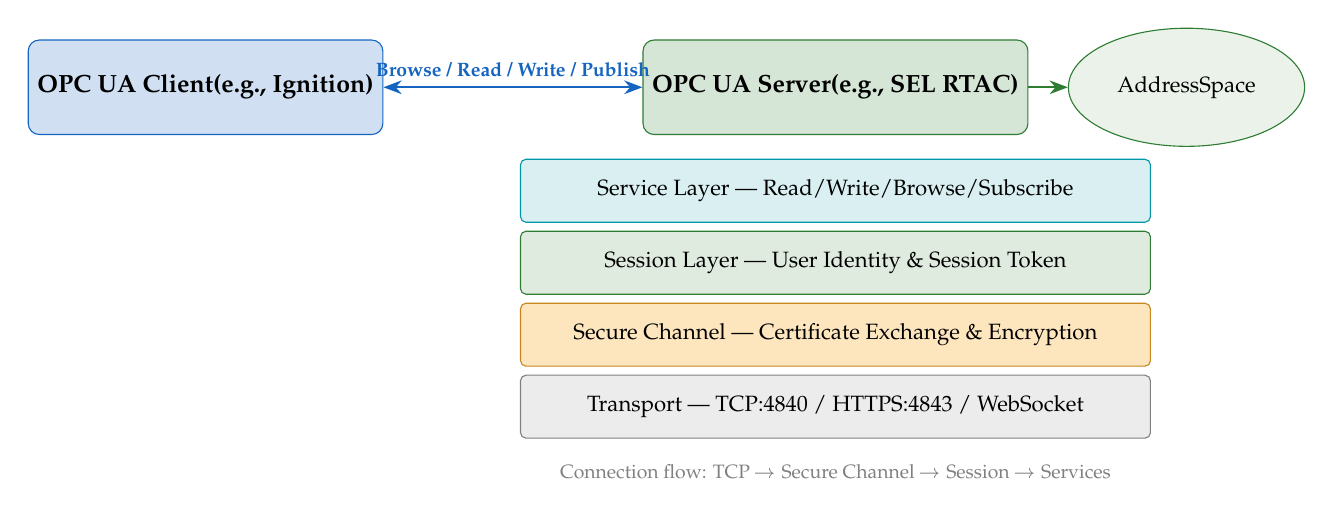
\begin{tikzpicture}[
  box/.style={rectangle, draw, rounded corners=4pt, minimum width=3cm, minimum height=1.2cm,
              text centered, font=\small\bfseries},
  layer/.style={rectangle, draw, rounded corners=2pt, minimum width=8cm, minimum height=0.8cm,
                text centered, font=\footnotesize},
  arrow/.style={-Stealth, thick},
  darrow/.style={Stealth-Stealth, thick},
]

% Client box
\node[box, fill=opcuablue!20, draw=opcuablue] (client) at (0, 4) {OPC UA Client\\(e.g., Ignition)};

% Server box
\node[box, fill=opcuagreen!20, draw=opcuagreen] (server) at (8, 4) {OPC UA Server\\(e.g., SEL RTAC)};

% Layer stack under server
\node[layer, fill=opcuacyan!15, draw=opcuacyan, below=0.3cm of server] (svc) {Service Layer — Read/Write/Browse/Subscribe};
\node[layer, fill=opcuagreen!15, draw=opcuagreen, below=0.1cm of svc] (sess) {Session Layer — User Identity \& Session Token};
\node[layer, fill=opcuayellow!30, draw=opcuayellow!80!black, below=0.1cm of sess] (sc) {Secure Channel — Certificate Exchange \& Encryption};
\node[layer, fill=gray!15, draw=gray, below=0.1cm of sc] (tcp) {Transport — TCP:4840 / HTTPS:4843 / WebSocket};

% Address space cloud
\node[ellipse, draw=opcuagreen, fill=opcuagreen!10, minimum width=3cm, minimum height=1.5cm,
      right=0.5cm of server, font=\footnotesize] (as) {Address\\Space};
\draw[arrow, opcuagreen] (server.east) -- (as.west);

% Arrows between client and server
\draw[darrow, opcuablue, thick] (client.east) -- node[above, font=\scriptsize\bfseries, text=opcuablue]
  {Browse / Read / Write / Publish} (server.west);

% Connection flow annotations
\node[font=\scriptsize, text=gray, below=0.2cm of tcp] {Connection flow: TCP → Secure Channel → Session → Services};

\end{tikzpicture}
\caption{OPC UA Client-Server Architecture with Layered Security Model}
\end{figure}

\section{Secure Channel Lifecycle}

\begin{lstlisting}[language=,caption={OPC UA Connection Sequence}]
CLIENT  ->  TCP Connect to server:4840
CLIENT  ->  OpenSecureChannel(SecurityMode, SecurityPolicy, ClientCert)
SERVER  <-  OpenSecureChannelResponse(ServerCert, SessionKeys)
CLIENT  ->  CreateSession(ClientCert, Endpoint)
SERVER  <-  CreateSessionResponse(SessionId, AuthToken)
CLIENT  ->  ActivateSession(UserIdentityToken)
SERVER  <-  ActivateSessionResponse(OK)
CLIENT  ->  Read / Browse / Subscribe  [all within Session]
\end{lstlisting}

\begin{fieldgotcha}
Certificate errors occur at \texttt{OpenSecureChannel} --- before any Session is created. If you see
\texttt{BadCertificateUntrusted}, the server received the client certificate but hasn't trusted it.
Fix: add the client cert to the server's trusted store, and add the server cert to the client's trusted store.
OPC UA is mutual authentication --- both sides must explicitly trust each other.
\end{fieldgotcha}

\section{Deployment Patterns}

\begin{description}
  \item[Embedded Server] OPC UA runs directly on the device (Siemens S7-1500, SEL RTAC, Beckhoff TwinCAT).
  \item[Gateway Server] Middleware connecting field devices and re-exposing them as OPC UA (Ignition, KEPServerEX).
  \item[Aggregation Server] Merges multiple OPC UA servers into one Address Space.
  \item[Historical Access Server] Exposes historian data via OPC UA Part 11 (Osisoft PI, etc.).
\end{description}

% =============================================================
\chapter{Information Model \& Address Space}
% =============================================================

The OPC UA Address Space is a browsable, typed graph of nodes. Every data point, every object, and every method
is a node. Nodes are connected by typed References.

\section{NodeId Formats}

Every node has a NodeId --- a unique identifier within a Namespace. Four formats exist:

\begin{tcolorbox}[title={NodeId Format Examples}, colback=codebg, colframe=opcuanavY!50!black, arc=4pt]
\begin{tabular}{ll}
\textbf{Format} & \textbf{Example} \\
\hline
Numeric  & \texttt{ns=2;i=1001} \\
String   & \texttt{ns=2;s=Temperature\_PV} \\
GUID     & \texttt{ns=2;g=550e8400-e29b-41d4-a716-446655440000} \\
Opaque   & \texttt{ns=2;b=AAEC} \\
\end{tabular}

\medskip
\textit{Namespace 0 (ns=0) is reserved for OPC UA specification nodes. Custom nodes use ns=1 or higher.
Numeric NodeIds are most common in auto-generated Address Spaces. String NodeIds are typical in human-readable
custom implementations.}
\end{tcolorbox}

\section{Node Classes}

\begin{tabularx}{\textwidth}{lXl}
\toprule
\textbf{Node Class} & \textbf{Purpose} & \textbf{Example} \\
\midrule
\rowcolor{rowlight} Object & Container — represents physical or logical entity & PLC, pump, device \\
Variable & Holds a typed value. Primary data node. & Temperature, speed \\
\rowcolor{rowlight} Method & Callable server-side function & StartPump() \\
ObjectType & Type definition for Objects (like a class) & PumpType \\
\rowcolor{rowlight} VariableType & Type with value constraints & AnalogItemType \\
ReferenceType & Semantic meaning of a node relationship & HasComponent \\
\rowcolor{rowlight} DataType & Data type for Variable values & Float, Structure \\
View & Pre-defined Address Space subset & Diagnostic view \\
\bottomrule
\end{tabularx}

\section{References}

Key reference types:
\begin{itemize}
  \item \texttt{HasComponent} --- Object HasComponent Variable/Method/Object
  \item \texttt{HasProperty} --- Descriptive attributes (engineering units, range)
  \item \texttt{Organizes} --- Folder-style grouping
  \item \texttt{HasTypeDefinition} --- Every Object/Variable has exactly one type
  \item \texttt{HasSubtype} --- Type inheritance
\end{itemize}

\begin{keyconcept}
Every Variable carries three things: a \textbf{Value}, a \textbf{StatusCode} (Good/Uncertain/Bad), and a
\textbf{SourceTimestamp}. A Bad StatusCode means the value is not trustworthy. SCADA systems must not display
Bad-status values as valid process data.
\end{keyconcept}

% =============================================================
\chapter{OPC UA Services}
% =============================================================

OPC UA defines 37 services in 11 service sets. All client-server interaction is a service call ---
a request/response pair with defined parameters and StatusCodes.

\section{Key Services}

\begin{tabularx}{\textwidth}{lXl}
\toprule
\textbf{Service Set} & \textbf{Key Services} & \textbf{Use Case} \\
\midrule
\rowcolor{rowlight} Discovery & FindServers, GetEndpoints & Server discovery \\
SecureChannel & OpenSecureChannel & Transport security \\
\rowcolor{rowlight} Session & CreateSession, ActivateSession & Connection management \\
View & Browse, TranslateBrowsePaths & Navigate Address Space \\
\rowcolor{rowlight} Attribute & Read, Write & Data access \\
Method & Call & Invoke server functions \\
\rowcolor{rowlight} MonitoredItem & CreateMonitoredItems & Set up monitoring \\
Subscription & CreateSubscription, Publish & Push data delivery \\
\bottomrule
\end{tabularx}

\section{Read vs. Subscribe}

\begin{tcolorbox}[title={Read vs Subscribe Comparison}, colback=white, colframe=opcuablue, arc=4pt]
\begin{tabular}{p{0.45\textwidth}p{0.45\textwidth}}
\textbf{Read (Polling)} & \textbf{Subscribe (Event-Driven)} \\
\hline
Client requests value every N ms & Server monitors and notifies on change \\
Network traffic $\propto$ poll rate $\times$ tags & Network traffic $\propto$ change rate \\
Always gets current value & Gets value when it changes \\
\textit{Use for: one-time reads, commissioning} & \textit{Use for: live SCADA, historian feed} \\
500 tags @ 500ms = 1000 req/sec & 500 tags, 3 changing = 3 notifications \\
\end{tabular}
\end{tcolorbox}

\begin{fieldgotcha}
Ignition uses subscriptions, not polling, for OPC UA tags. When you create an OPC UA tag in Ignition, it
creates a MonitoredItem in a Subscription. This is why Ignition is more network-efficient than Modbus TCP
polling for large tag counts.
\end{fieldgotcha}

% =============================================================
\chapter{Security \& Certificates}
% =============================================================

OPC UA has well-designed security: mutual certificate authentication, encrypted sessions, signed messages.
The practical problem: 90\% of OPC UA deployments use \texttt{SecurityMode=None} because certificate
configuration is hard and the deadline was yesterday.

\section{SecurityMode Comparison}

\begin{tcolorbox}[title={SecurityMode Comparison}, colback=white, colframe=opcuanavy, arc=4pt]
\begin{tabular}{p{3.5cm}p{3.5cm}p{3.5cm}p{1.5cm}}
\toprule
 & \textbf{None} & \textbf{Sign} & \textbf{Sign\&Encrypt} \\
\midrule
\rowcolor{securityred} Message Signing & \texttimes & \checkmark & \checkmark \\
\rowcolor{securityred} Encryption & \texttimes & \texttimes & \checkmark \\
\rowcolor{rowlight} Certificates Required & No & Yes (both) & Yes (both) \\
\rowcolor{securityred} Traffic Readable & Yes & Yes & No \\
\rowcolor{securitygreen} Suitable for Production & No & Marginal & \textbf{Yes} \\
\bottomrule
\end{tabular}
\end{tcolorbox}

\section{Certificate Trust Workflow}

\begin{enumerate}
  \item Server generates self-signed X.509 certificate on first startup
  \item Client connects, receives server certificate
  \item Client checks its trusted store --- if not found: \texttt{BadCertificateUntrusted}
  \item Client also presents its certificate (mutual auth)
  \item Server checks its trusted store --- if not found: connection rejected
  \item Both sides must explicitly trust each other's certificates
\end{enumerate}

\begin{warningbox}
\texttt{SecurityMode=None} means all OPC UA traffic is unencrypted and unsigned. Any device on the control
network can read process data. On a network with any external connectivity, this is a critical vulnerability.
\end{warningbox}

\section{Security Policies}

Use \textbf{Basic256Sha256} as the minimum acceptable security policy. Basic128Rsa15 and Basic256 use SHA-1
(broken) and are deprecated. The Aes256\_Sha256\_RsaPss policy provides the highest currently available security.

% =============================================================
\chapter{Subscriptions \& MonitoredItems}
% =============================================================

A Subscription is a container on the server. MonitoredItems are the data points being watched inside it.
The server samples MonitoredItems at the SamplingInterval and sends notifications to the client at the
PublishingInterval.

\section{Key Parameters}

\begin{tabularx}{\textwidth}{lXr}
\toprule
\textbf{Parameter} & \textbf{Description} & \textbf{Typical} \\
\midrule
\rowcolor{rowlight} PublishingInterval & Rate at which server delivers notifications (ms) & 500--5000 ms \\
LifetimeCount & Sessions before subscription deleted without Publish & 3$\times$MaxKeepAlive \\
\rowcolor{rowlight} MaxKeepAliveCount & Empty intervals before KeepAlive sent & 10 \\
SamplingInterval & Per-item: how fast server samples source (ms) & 100--1000 ms \\
\rowcolor{rowlight} QueueSize & Per-item: notification buffer depth & 1--10 \\
\bottomrule
\end{tabularx}

\begin{keyconcept}
SamplingInterval can be faster than PublishingInterval. The server samples data into a queue at SamplingInterval
and delivers the accumulated notifications at PublishingInterval. QueueSize controls how many samples are
buffered between deliveries.
\end{keyconcept}

\section{Deadband Filtering}

\begin{description}
  \item[Absolute Deadband] Suppress if $|$new -- old$|$ $<$ deadband. Example: only notify if temperature changes by more than 0.5°C.
  \item[Percentage Deadband] Suppress if change $<$ X\% of the EURange. Requires EURange property on the Variable.
\end{description}

% =============================================================
\chapter{Transport \& Encoding}
% =============================================================

OPC UA separates the data model from the transport. Three transport mappings are defined.

\section{Transport Comparison}

\begin{tabularx}{\textwidth}{lllX}
\toprule
\textbf{Transport} & \textbf{Port} & \textbf{Encoding} & \textbf{Notes} \\
\midrule
\rowcolor{rowlight} UA-TCP Binary & 4840 & Binary & Fastest, most common, use this \\
HTTPS & 4843 & Binary or JSON & For IT/OT integration, proxies \\
\rowcolor{rowlight} WebSocket & 4840/443 & Binary or JSON & Browser clients, rarely needed \\
\bottomrule
\end{tabularx}

\section{Binary Encoding Built-In Types}

OPC UA defines 25 built-in types. Key ones: Boolean (1 byte), Int32 (4), Float (4), Double (8), String (4+N),
DateTime (8 bytes, 100-nanosecond ticks since 1601-01-01), StatusCode (4), NodeId (variable), Variant (type+value),
DataValue (value+status+timestamps), ExtensionObject (any type).

\begin{protip}
The \texttt{Variant} type can hold any built-in type plus arrays. Variable values are transmitted as Variants.
This allows OPC UA's heterogeneous Address Space to use a single serialization format for all data types.
\end{protip}

% =============================================================
\chapter{OPC UA in Ignition \& RTAC}
% =============================================================

Ignition is simultaneously an OPC UA server (exposes tags to external clients on port 62541) and an OPC UA
client (connects to PLCs and RTACs to read process data).

\section{Ignition OPC UA Client Workflow}

\begin{enumerate}
  \item Gateway $\to$ OPC UA $\to$ Connections $\to$ Add connection
  \item Enter server endpoint URL (\texttt{opc.tcp://192.168.1.100:4840})
  \item First connect attempt downloads server certificate to Quarantine folder
  \item Trust the server certificate: Gateway $\to$ OPC UA $\to$ Certificates $\to$ Quarantined $\to$ Trust
  \item Export Ignition's client certificate and import it into the server's trusted store
  \item Connection status should change to Connected
\end{enumerate}

\begin{fieldgotcha}
The most common commissioning mistake: trusting the server certificate in Ignition but forgetting that the
server also needs to trust Ignition's certificate. OPC UA is mutual authentication. Both sides trust both
certificates. If you've done only one side, the connection fails from the server's perspective.
\end{fieldgotcha}

\section{SEL RTAC as OPC UA Server}

The SEL RTAC includes a built-in OPC UA server (AcSELerator RTAC $\to$ Communications $\to$ OPC UA Server).
It generates a self-signed certificate. The RTAC must trust Ignition's client certificate; Ignition must trust
the RTAC's server certificate. Both certificates are self-signed --- the PKI trust is entirely manual.

% =============================================================
\chapter{Troubleshooting OPC UA}
% =============================================================

OPC UA provides specific status codes for every failure mode. The diagnostic ladder: ping $\to$ port check
$\to$ service running $\to$ UA Expert with SecurityMode=None $\to$ specific error code.

\section{Common Status Codes}

\begin{tabularx}{\textwidth}{lXl}
\toprule
\textbf{Status Code} & \textbf{Cause and Fix} & \textbf{When} \\
\midrule
\rowcolor{rowlight} \texttt{BadCertificateUntrusted} & Certificate not in trusted store. Trust on both sides. & OpenSecureChannel \\
\texttt{BadSecureChannelClosed} & Channel closed by server (restart, timeout, cert expiry). Reconnect. & During session \\
\rowcolor{rowlight} \texttt{BadNodeIdUnknown} & NodeId doesn't exist. Verify via Browse. Check namespace index. & Read/Write \\
\texttt{BadUserAccessDenied} & User lacks permission or wrong credentials. & ActivateSession \\
\rowcolor{rowlight} \texttt{BadSubscriptionIdInvalid} & Subscription deleted (session loss). Recreate subscription. & Publish \\
\texttt{BadTooManySubscriptions} & Server subscription limit reached. Delete unused subscriptions. & CreateSubscription \\
\bottomrule
\end{tabularx}

\section{UA Expert Diagnostic Workflow}

\begin{enumerate}
  \item Connect with SecurityMode=None --- if this works, it's a security/certificate issue
  \item Browse the Address Space --- verify NodeIds before writing client code
  \item Subscribe to nodes in Data Access View --- verify data is changing
  \item Check Connection Log for exact error codes
  \item Certificate dialog for trust management
\end{enumerate}

% =============================================================
\chapter{Lab \& Tools}
% =============================================================

\section{Required Tools (All Free)}

\begin{tabularx}{\textwidth}{llX}
\toprule
\textbf{Tool} & \textbf{Provider} & \textbf{Use} \\
\midrule
\rowcolor{rowlight} UA Expert & Unified Automation & OPC UA diagnostic client --- the Wireshark of OPC UA \\
Prosys Simulation Server & Prosys OPC Ltd & Full OPC UA server with simulated process data \\
\rowcolor{rowlight} Node-RED OPC UA & npm / flows.nodered.org & Flow-based OPC UA client, no coding required \\
opcua-asyncio (Python) & PyPI (pip install asyncua) & Full Python OPC UA client and server library \\
\bottomrule
\end{tabularx}

\section{Lab Exercises}

\begin{enumerate}
  \item \textbf{Basic Connection}: Install Prosys + UA Expert. Connect with SecurityMode=None. Browse address space.
  \item \textbf{Subscribe}: Add sinusoidal nodes to Data Access View. Change sampling intervals. Observe behavior.
  \item \textbf{Security}: Configure Prosys for SignAndEncrypt. Complete the mutual certificate trust workflow.
  \item \textbf{Python Client}: Write a script using opcua-asyncio. Connect, read, subscribe, write.
  \item \textbf{Ignition + Prosys}: Connect Ignition to Prosys. Complete the full certificate trust workflow on both sides.
\end{enumerate}

\begin{protip}
Complete Lab Exercise 5 before commissioning any real OPC UA device in Ignition. The certificate trust workflow
is identical regardless of whether the server is Prosys or an SEL RTAC. Practicing in the lab means
commissioning takes 10 minutes instead of an hour.
\end{protip}

\section{Professional Certification Context}

No individual exam-based credential currently exists specifically for OPC UA. Practitioners in industrial automation who work with OPC UA typically pursue:

\begin{itemize}
\item \textbf{ISA CCST} (Certified Control Systems Technician) --- covers industrial communications protocols, PID control, SCADA integration, and field instrumentation. Levels I, II, and III based on experience. See isa.org/certification/ccst.
\item \textbf{ISA CAP} (Certified Automation Professional) --- broader engineering credential covering process control, automation systems, and integration. Requires engineering background. See isa.org/certification/cap.
\item \textbf{Vendor-Specific Context}:
  \begin{itemize}
  \item For Modbus: Inductive Automation Core/Gold certification tests Modbus connectivity in Ignition context.
  \item For DNP3: Triangle Microworks and SEL University offer training (PDHs, not credentials).
  \item For OPC UA: MatrikonOPC OPCSI is a vendor-sponsored credential for OPC systems integrators.
  \item For IEC 61131-3: Vendor-specific certs (Rockwell, Siemens, Beckhoff) test platform-specific implementations. SEL University APP RTAC ADV-1 covers IEC 61131-3 in RTAC context.
  \item For RTAC: SEL University APP RTAC course awards PDHs. No formal credential exam.
  \end{itemize}
\end{itemize}

\end{document}
